\section{Related Work}
\siyu{I think the classification of related works in Pixel2Mesh++ is more reasonable, that is 3D shape representation, single-view shape generation, and multi-view shape generation.
The ``Traditional Shape Generation Methods'' can be merged into ``single-view shape generation'' and ``multi-view shape generation''. We donot have to survey ``Depth Estimation'', which seems irrelevant to our approach.}

\textcolor{Red}{
\paragraph{3D Shape Representation.} 
We can discuss about:
1. Different representations of 3D shape in learning-based approaches. Please refer to the survey in Pixel2Mesh++.
2. The existed works of initial mesh generation, and especially the limitations of such methods and the effect of initial mesh on the final results.
3. To overcome such limitations, we use the voxel grid as the 3D representation of the initial mesh, and multi-view ... to obtain the initial mesh.
\paragraph{Single-view Shape Generation.} 
Point cloud, voxel grid and mesh... Maybe we can mainly focus on the voxel grid and mesh.
\paragraph{Multi-view Shape Generation.}
Mainly focus on the limitations of existed methods and how can we handle such limitations.
}

\begin{figure*}[t]
\begin{center}
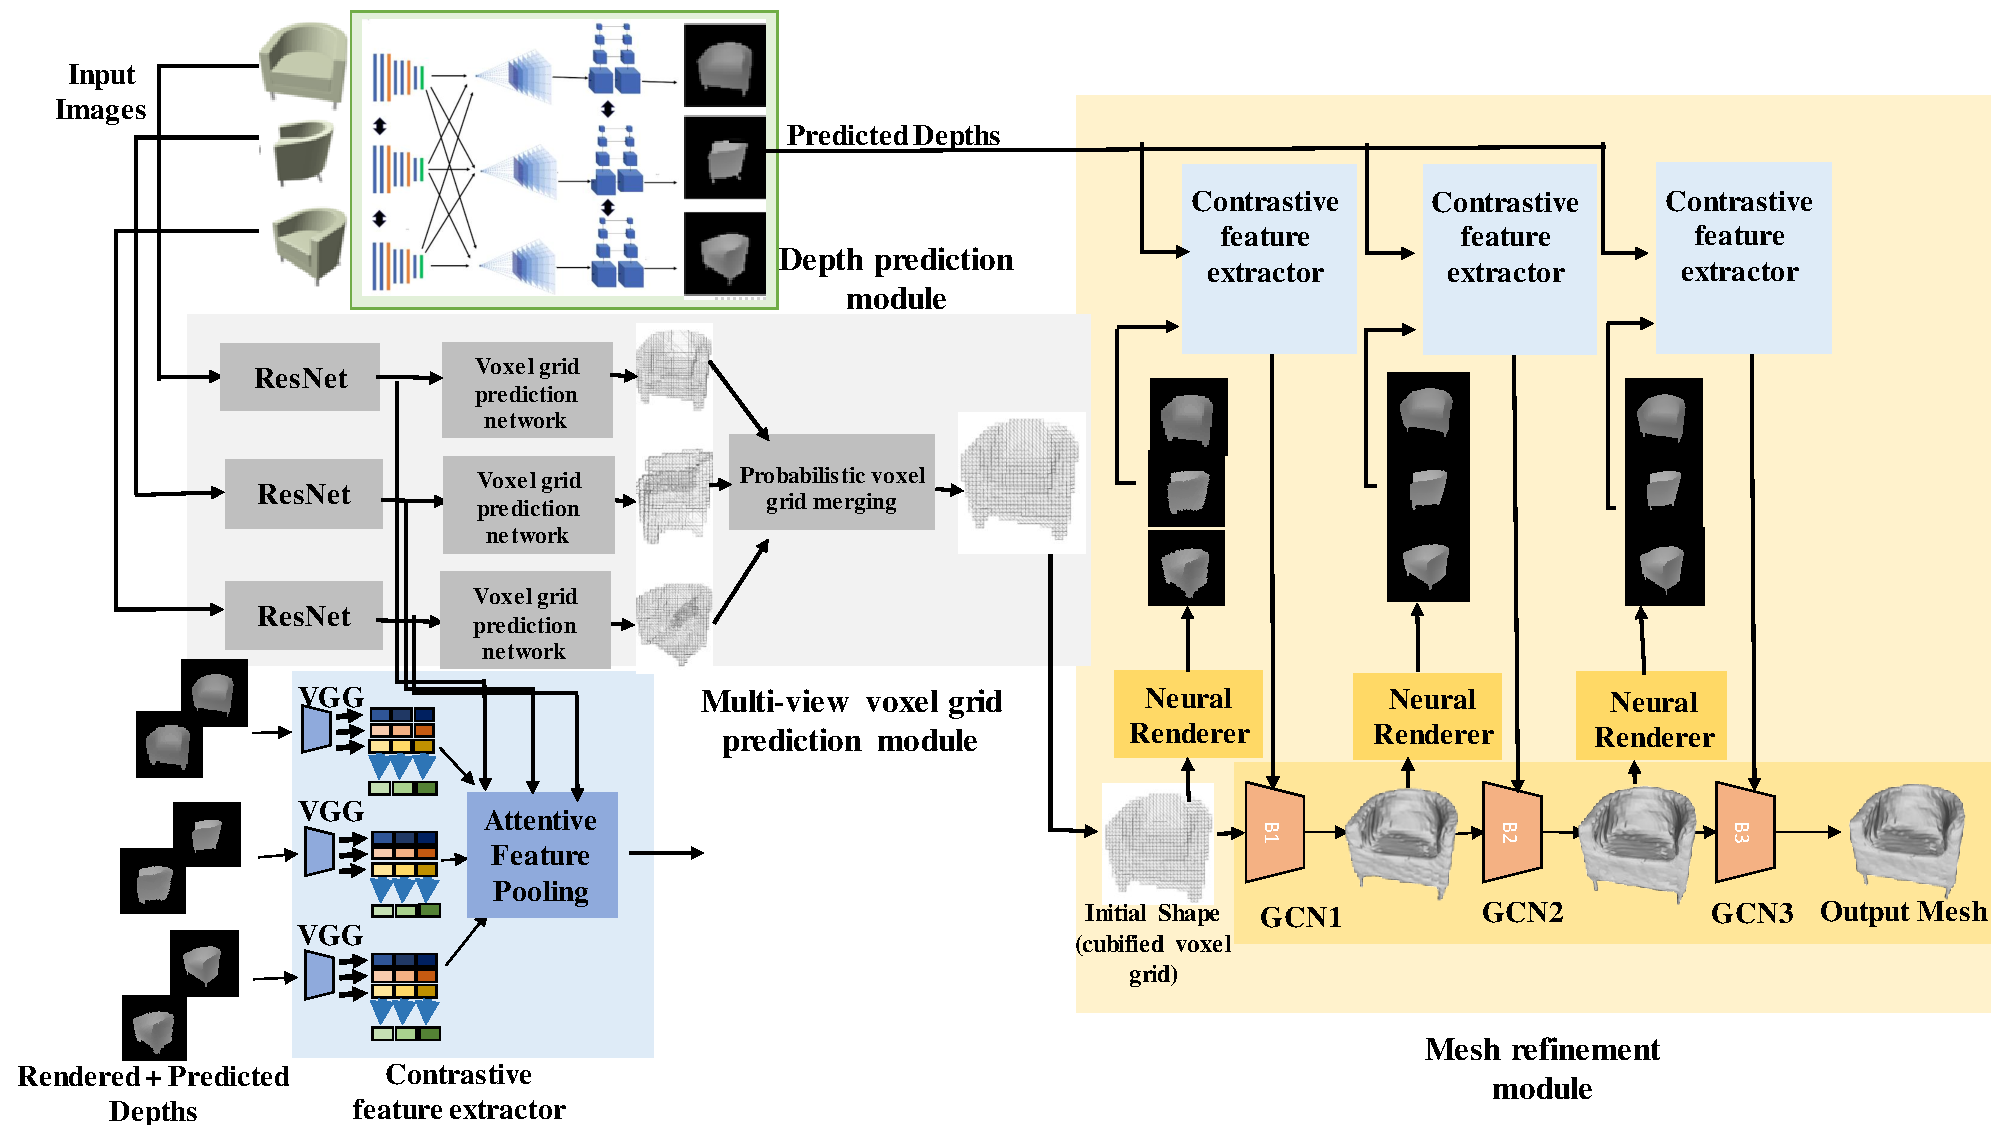
\includegraphics[width=\linewidth]{imgs/meshrcnn_architecture.pdf}
\end{center}
\caption{
    \textbf{Architecture of the proposed method}.
    The \emph{voxel grid prediction module} predicts coarse voxel grid representation by using CNN to predict voxel grids for each input image and then probabilistically merging them.
    A series of \emph{GCN}s further refine the cubified voxel grid in a coarse-to-fine manner
    using \emph{contrastive depth features} from rendered depths of the current shape and the predicted depths from \emph{depth prediction module} along with RGB image features.
    Multi-view features are pooled using a attention-based mechanism.
    \siyu{Replace this figure with a simplified one and add a long caption describing the whole framework.}
    \rakesh{simplified figure has been placed and caption has been expanded}
}
\label{fig:system_architecture}
\end{figure*}

\paragraph{Traditional Shape Generation Methods}
3D model generation has traditionally been tackled using multi-view geometry principles.
Among them, structure-from-motion (SfM)~\cite{schonberger2016structure,agarwal2011building,cui2015global,cui2017hsfm} and simultaneous localization and mapping (SLAM)~\cite{cadena2016pastslam,mur2015orb,engel2014lsd,whelan2015elasticfusion} are popular techniques that perform 3D reconstruction and camera pose estimation at the same time. These methods extract local image features, match them across images and use the matches to estimate camera poses and 3D geometry.
% But these methods are limited to texture-rich objects with non-reflective surfaces
% and optimal/exhaustive view selection is also essential for reconstructing a complete 3D model with high accuracy.
Closer to our problem setup, multi-view stereo methods infer 3D geometry from images with known camera parameters.
% These generally fall into one of two categories: Volumetric and Point Cloud based methods.
Volumetric methods~\cite{kar2017lsm, kutulakos2000theory, seitz1999photorealistic} predict voxel grid representation of objects by estimating the relationship between each voxel and object surfaces.
Point cloud based methods~\cite{furukawa2009accurate, lhuillier2005quasi} start with a sparse point cloud and
gradually increase the density of points to obtain a final dense point cloud of the object.
\cite{durou2008numerical,zhang1999shape,favaro2005geometric} reason about shading, texture and defocus to reason about visible parts of the object and infer its 3D geometry.
While the results of these works are impressive in terms of quality and completeness of reconstruction, they still struggle with poorly textured and reflective surfaces and require carefully selected input views.

\paragraph{Deep Shape Generation Methods}
 Deep learning based approaches can learn to infer 3D structure from training data and can be robust against poorly textured and reflective surfaces as well as limited and arbitrarily selected input views. These methods can be categorized into single view and multi-view methods.
\cite{huang2015single, su2014estimating} use shape component retrieval and deformation from a large dataset for single-view 3D shape generation.
\cite{kurenkov2018deformnet} extend this idea by introducing free-form deformation networks on retrieved object templates from a database.
Some work learn shape deformation from ground truth foreground masks of 2D images~\cite{kar2015category,yan2016perspective,tulsiani2017multi}.
Recurrent Neural Networks (RNN) based methods~\cite{3dr2n2, kar2017lsm, mcrecon2017} are another popular solution to solve this problem.
\cite{mcrecon2017, lin2019photometric} introduce image silhouettes along with adversarial multi-view constraints and optimize object mesh models using multi-view photometric constraints.
Predicting mesh directly from color images was proposed in~\cite{wang2018pixel2mesh, wickramasinghe2019voxel2mesh,pan2019deep,wen2019pixel2mesh++, gkioxari2019meshrcnn, tang2019skeleton}.
DR-KFS~\cite{jin2019drkfs} introduces a differentiable visual similarity metric
while SeqXY2SeqZ~\cite{han2020seqxy2seqz} represents 3D shapes using a set of 2D voxel tubes for shape reconstruction.
Front2Back~\cite{yao2020front2back} generates 3D shapes by fusing predicted depth and normal images and
DV-Net~\cite{jia2020dv} predicts dense object point clouds using dual-view RGB images with a gated control network to fuse point clouds from the two views.
FoldingNet~\cite{yang2018foldingnet} learns to reconstruct arbitrary point clouds from a single 2D grid.
AtlasNet~\cite{groueix2018papier} use learned parametric representation
while \cite{mescheder2019occupancy,park2019deepsdf,liu2019learning,liu2019dist,murez2020atlas} employ implicit surface representation to reconstruct 3D shapes.

% Pixel2Mesh~\cite{wang2018pixel2mesh} utilizes a single image of an object to predict its triangle mesh using perceptual features extracted from the image as GCN input.
% Voxel2Mesh~\cite{wickramasinghe2019voxel2mesh} extends Pixel2Mesh by using 3D volumes as input instead of 2D images.
% Pan et al.~\cite{pan2019deep} propose a similar progressive framework which alternates between neural networks for mesh deformation and topology modification for pruning error-prone faces.
% DR-KFS~\cite{jin2019drkfs} introduces a differentiable visual similarity metric for improving reconstruction quality of various shape generation methods.
% SeqXY2SeqZ~\cite{han2020seqxy2seqz} represent 3D shapes using a set of 2D voxel tubes which are predicted using RNN with a single image as input.
% Front2Back~\cite{yao2020front2back} generate 3D shapes by fusing predicted depth and normal images using Screen Poisson surface reconstruction~\cite{kazhdan2013screened}.
% Mesh R-CNN~\cite{gkioxari2019meshrcnn} utilizes instance segmentation to predict a coarse voxel grid which is further refined using GCNs to obtain a mesh from a single image.
% \cite{tang2019skeleton} further break down shape generation into skeleton prediction followed by voxel grid generation and finally GCN based mesh refinement.

% Recurrent Neural Networks (RNN) have been a popular solution for multi-view 3D reconstruction.
% 3D-R2N2~\cite{3dr2n2} employs 3D RNN with encoder-decoder architecture
% while LSM~\cite{kar2017lsm} uses recurrent 3D features grid fusion to predict 3D occupancy grid models.
% Gwak et al.~\cite{mcrecon2017} use image silhouettes along with adversarial multi-view constraints to estimate 3D voxel grid models.
% \cite{lin2019photometric} optimizes object mesh models using multi-view photometric constraint by piecewise image alignment of each mesh faces' rasterized projections.
% Pixel2Mesh++~\cite{wen2019pixel2mesh++} uses feature statistics from multi-view images to refine the mesh generated by Pixel2Mesh by further deforming the mesh vertices within a local neighborhood.

% We refer our readers to a recent survey on Deep Geometry Learning ~\cite{xiao2020survey} for a more comprehensive review of the related work on this topic.

\paragraph{Depth Estimation}
Compared to 3D shape generation, depth prediction is an easier problem formulation since it simplifies the task to per-view depth map estimation.
Traditional methods ~\cite{campbell2008using,galliani2015massively,schonberger2016pixelwise} use multi-view stereo principles for depth prediction.
Deep learning based multi-view stereo depth estimation was first introduced in~\cite{hartmann2017learned_16} where a learned cost metric is used to estimate patch similarities.
DeepMVS~\cite{deepmvs2018} warps multi-view images to 3D space and then applies deep networks for regularization and aggregation to estimate depth images.
Learned 3D cost volume based depth prediction was proposed in MVSNet~\cite{yao2018mvsnet} where a 3 dimensional cost volume is built using homographically warped 2D features from multi-view images and 3D CNNs are used for cost regularization and depth regression.
This idea was further extended by~\cite{chen2019point,luo2019pmvsnet, gu2019cascade,yao2019recurrent}.

% Our system aims to combine the strengths of GCN based methods and depth prediction methods to improve the accuracy of the 3D structure while still ensuring completeness.
